%==============================================================================
%  Strict-Bound Verification for Document-Grounded Exam Generation
%  APA 7th edition manuscript  ·  SEGS project
%
%  BUILD:  latexmk -pdf strict_bound_verification.tex
%          (or upload this file + references.bib to Overleaf and press Recompile)
%
%  EDIT BEFORE SUBMITTING: the five \author / \affiliation / \course /
%  \professor / \duedate lines marked TODO below.
%==============================================================================

% Class options:
%   stu = student paper (course, instructor, due date on title page)
%   man = manuscript      jou = typeset journal article
\documentclass[stu,11pt,floatsintext]{apa7}

\usepackage[american]{babel}
\usepackage{csquotes}
\usepackage[style=apa,backend=biber]{biblatex}
\DeclareLanguageMapping{american}{american-apa}
\addbibresource{references.bib}

\usepackage{amsmath}
\usepackage{booktabs}
\usepackage{array}
\usepackage{ragged2e}
\usepackage{pgfplots}
\pgfplotsset{compat=1.18}
\usepackage[hidelinks]{hyperref}

\newcolumntype{L}[1]{>{\RaggedRight\arraybackslash}p{#1}}

%------------------------------------------------------------------ TODO ------
\title{Strict-Bound Verification for Document-Grounded Exam Generation}
\shorttitle{Strict-Bound Verification}
\author{Author Name}                                    % TODO
\affiliation{Department, University}                    % TODO
\course{Course Code: Course Title}                      % TODO
\professor{Instructor Name}                             % TODO
\duedate{September 9, 2026}                             % TODO
%------------------------------------------------------------------------------

\abstract{%
The Smart Exam Generator System (SEGS) generates examination items from
user-uploaded curriculum documents and claims to eliminate model hallucination
through strict context bounding. That bounding is presently enforced by prompt
instruction alone, and the system's groundedness flags record the generating
model's own assessment of its output rather than any independent check. This
report specifies the machinery required to convert that claim into a measured
quantity. We define a \emph{strict-bound rate} (SBR) as the conjunction of four
item-level checks---citation validity, answer groundedness, distractor
soundness, and span verifiability---and specify a five-layer verification
architecture ordered by cost per item, from deterministic string checks through
natural language inference verification to selective model adjudication. We show
that groundedness improves not because verification corrects items but because
over-generation permits discarding them, and we give the filtering arithmetic
that maps per-layer catch and false-flag rates onto an achievable SBR and its
attendant yield cost. Under working targets drawn from published detector
performance, a 90.0\% baseline reaches 99.4\% at a yield of 83.4\%. We identify
two ways this arithmetic misleads---correlated gate failures and circular
self-measurement---and specify a calibration protocol, including sample-size
requirements, under which a 99\% claim becomes statistically defensible.
}

\keywords{hallucination detection, natural language inference, automatic question
generation, retrieval-augmented generation, educational assessment}

\begin{document}
\maketitle

%==============================================================================
\section{The Claim and the Gap}

SEGS transforms uploaded curriculum documents into interactive examinations. Its
product specification states that the system ``eliminates AI hallucination
entirely'' by confining generation to the uploaded context and attaching
paragraph-level citations to every item.

In the current implementation, that confinement is enforced entirely through
prompt instruction. The generation prompt forbids the use of outside knowledge
and requires a citation field, and the system stores two boolean flags,
\texttt{curriculumAligned} and \texttt{outOfBounds}, alongside each generated
item. Both flags are populated from the generating model's own report about its
own output, defaulting to \texttt{true} and \texttt{false} respectively when the
model omits them. No component of the pipeline verifies either flag, and no
component checks that a cited paragraph code resolves to a paragraph that
exists. The educator-facing audit panel, which displays out-of-bounds counts and
an alignment rate, therefore reads values that are structurally incapable of
indicating a problem.

The magnitude of the gap can be estimated from published measurements.
\textcite{vectara2025leaderboard} evaluate frontier models on grounded
summarization: a model receives a source article and produces a summary, and
hallucination is scored as the proportion of summaries an entailment model rates
below 0.5. On the November 2025 revision of that benchmark---more than 7,700
articles of up to 32,000 tokens across ten domains---the best-performing model
recorded a 3.3\% hallucination rate, and most frontier models exceeded 10\%.

Grounded summarization is strictly easier than grounded question generation.
Summarization requires only restatement of source content; question generation
requires restatement together with a correct answer, a set of distractors that
must all be false, and a citation that must resolve. A system that performs no
verification cannot claim a groundedness rate better than the underlying model's
performance on the easier task.

\subsection{The Structural Advantage}

One asymmetry works decisively in favour of exam generation. A summarization
system must emit an output for every input. An exam generation system need not:
if a candidate item fails verification, it can be discarded and another
generated in its place. Groundedness therefore improves not because verification
repairs defective items but because over-generation makes discarding them
affordable. This asymmetry is the organising principle of the architecture
proposed below, and it is why rates unattainable in summarization are reachable
here.

%==============================================================================
\section{Defining the Strict-Bound Rate}

A rate cannot be reported before it is defined. We adopt the claim-decomposition
approach that has become standard in retrieval-augmented generation evaluation,
in which an output is split into atomic claims and each claim is checked against
the evidence it cites \parencite{es2024ragas}. For an examination item the atoms
are supplied by the schema rather than requiring extraction.

\subsection{Four Item-Level Checks}

Let $Q$ be a set of generated items, $P$ the set of stored source paragraphs,
$\mathrm{cite}(q)$ the paragraph code an item cites, $\mathrm{chunk}(q)$ the text
of that paragraph, $\mathrm{stem}(q)$ the question text, $\mathrm{ans}(q)$ the
correct answer, and $D(q)$ the distractor set.

\subsubsection{M1: Citation Validity} The cited paragraph must exist and must
support the item. This is citation recall in the sense of
\textcite{gao2023enabling}, who validate automatic citation scoring against human
judgement at 85.1\% accuracy for recall and 77.6\% for precision. An item citing
\texttt{P9} in a four-paragraph document fails unconditionally.
\begin{equation}
\mathrm{CV} = \frac{\bigl|\{q \in Q : \mathrm{cite}(q) \in P \wedge \mathrm{entails}(\mathrm{chunk}(q), q)\}\bigr|}{|Q|}
\end{equation}

\subsubsection{M2: Answer Groundedness} The stem and its answer are fused into a
single declarative claim and tested for entailment against the cited paragraph
alone. This is the load-bearing check.
\begin{equation}
\mathrm{AG} = \frac{\bigl|\{q \in Q : \mathrm{entails}(\mathrm{chunk}(q),\; \mathrm{stem}(q) \oplus \mathrm{ans}(q))\}\bigr|}{|Q|}
\end{equation}

\subsubsection{M3: Distractor Soundness} Every distractor must be false with
respect to the source. A distractor the source also supports produces a second
correct key and renders the item unanswerable---a failure mode the
distractor-generation literature treats as central and automated pipelines
routinely omit \parencite{alhazmi2024distractor}.
\begin{equation}
\mathrm{DS} = \frac{\bigl|\{q \in Q_{\mathrm{mc}} : \forall d \in D(q),\; \neg\,\mathrm{entails}(\mathrm{chunk}(q),\; \mathrm{stem}(q) \oplus d)\}\bigr|}{|Q_{\mathrm{mc}}|}
\end{equation}

\subsubsection{M4: Span Verifiability} For fill-in-the-blank and cloze
multiple-choice items the answer must occur verbatim in the source. This is pure
string containment: no model, no inference cost, and no error.
\begin{equation}
\mathrm{SV} = \frac{\bigl|\{q \in Q_{\mathrm{ext}} : \mathrm{ans}(q) \subseteq \mathrm{chunk}(q)\}\bigr|}{|Q_{\mathrm{ext}}|}
\end{equation}

\subsection{The Composite Metric}

The headline figure is the conjunction of all applicable checks, not their
average:
\begin{equation}
\mathrm{SBR} = \frac{\bigl|\{q \in Q : M_1(q) \wedge M_2(q) \wedge M_3(q) \wedge M_4(q)\}\bigr|}{|Q|}
\end{equation}

Averaging would allow an item with an unresolvable citation to score 75\%.
Conjunction is what \emph{strict} denotes: one failed check, one failed item. It
yields a lower and more defensible headline number, and it is the only
formulation consistent with the product claim.

%==============================================================================
\section{A Layered Verification Architecture}

Table~\ref{tab:layers} specifies five layers ordered by cost per item. Each runs
only on items that survived the preceding layer, so expensive models process a
small fraction of total traffic. \emph{Catch rate} denotes the proportion of
ungrounded items a layer removes; \emph{false-flag rate} the proportion of sound
items it wrongly rejects. Both are quantities to be measured on a
project-specific calibration set; the values given are the working targets
assumed by the arithmetic in the following section.

\begin{table}[htbp]
\caption{Verification Layers Ordered by Cost per Item}
\label{tab:layers}
\begin{tabular}{@{}l L{4.6cm} l l l@{}}
\toprule
Layer & Function & Cost/item & Catch & False flag \\
\midrule
L0 & Context integrity: verify every paragraph code resolves to stored text before generation & 0 & --- & --- \\
L1 & Constrained generation: one chunk per call, JSON schema with mandatory citation and verbatim evidence span & 1 call & --- & --- \\
L2 & Deterministic gates: citation resolution, span containment, option distinctness, single-key check & $\approx$ 0 ms & 45\% & 1\% \\
L3 & Entailment verification: dedicated factual-consistency model scores claim against cited chunk & 50--200 ms & 80\% & 5\% \\
L4 & Adjudication: second model on the uncertain band only; failures dropped and regenerated & 1 call, $\approx$15\% of items & 55\% & 2\% \\
\bottomrule
\end{tabular}
\par\vspace{0.5em}
\footnotesize\textit{Note.} Catch and false-flag values are working targets, not
measurements. They must be re-estimated on a project-specific calibration set
before any rate derived from them is reported.
\end{table}

\subsection{L0--L1: Raising the Floor}

Context integrity is already largely satisfied in SEGS. The existing chunker
segments documents into typed structural blocks, keeps tables whole with
repeated headers, and never divides a sentence, list item, or formula
mid-span---a claim can only be verified against evidence that survived
extraction intact. The addition required is an assertion that every paragraph
code resolves to stored text before generation begins.

Constrained generation raises the baseline before verification runs. Sending one
chunk per call rather than the entire document makes the citation structurally
determined rather than model-selected. Requiring a JSON schema containing a
mandatory citation and an \texttt{evidence\_span} that the model must copy
verbatim from the chunk yields a field checkable by string containment. These
are prompt-level measures: they move the baseline by a few points and cannot be
relied upon beyond that, because prompt instructions are requests rather than
constraints.

\subsection{L2: Deterministic Gates}

The cheapest layer involves no model, no latency, and no inference error. The
checks are: the citation code resolves to a real paragraph; the
\texttt{evidence\_span} occurs verbatim in that paragraph; for cloze items the
answer occurs verbatim (M4); options are distinct after normalisation; the key
appears among the options; exactly one blank exists; and no option is a
substring of the stem. This layer should be built first. It converts
\texttt{outOfBounds} from a decorative field into a measurement at zero
inference cost.

\subsection{L3: Entailment Verification}

The load-bearing layer applies a dedicated factual-consistency model---not the
generator---to score the fused stem-and-answer claim against the cited chunk,
and to score every distractor for the M3 check. Candidate models are compared in
Table~\ref{tab:verifiers}. The decision threshold must be tuned on a
project-specific labelled set rather than inherited from a model card.

\subsection{L4: Adjudication and Repair}

A second model runs only on the uncertain band---entailment scores between
approximately 0.35 and 0.75---bounding cost. Chain-of-Verification supplies the
pattern: draft a response, plan verification questions, answer those questions
independently of the draft, then revise \parencite{dhuliawala2024chain}.
Independence is the active ingredient; a model re-reading its own draft largely
agrees with it. Items that still fail are discarded and regenerated rather than
displayed.

A caution applies to model-based adjudication. Judge models agree with human
raters at approximately the rate at which human raters agree with one another,
but carry documented biases: position preference of up to 75\% toward the
first-listed option, and self-enhancement bias of 10--25\% toward text generated
by the same model family \parencite{gu2024survey}. Mitigations are to use a
different model family than the generator, randomise option order, and calibrate
the judge against human labels before relying on it.

%==============================================================================
\section{Quantifying the Effect of Filtering}

Verification does not raise groundedness; it labels it. The rate rises because
over-generation permits discarding. Let $G_i$ and $B_i$ denote the surviving
mass of grounded and ungrounded items after layer $i$, $f_i$ the layer's
false-flag rate, and $r_i$ its catch rate:
\begin{align}
G_i &= G_{i-1}\,(1 - f_i) \\
B_i &= B_{i-1}\,(1 - r_i) \\
\mathrm{SBR}_i &= \frac{G_i}{G_i + B_i}, \qquad
\mathrm{yield}_i = G_i + B_i
\end{align}

Figure~\ref{fig:filtering} traces both quantities through the stack from a
90.0\% raw baseline, using the working targets of Table~\ref{tab:layers}.
Delivering 20 verified items requires generating 24. The residual defect rate at
the end of the stack is 0.6\%, or approximately one flawed item per 168 shipped.

\begin{figure}[htbp]
\caption{Strict-Bound Rate and Yield Across Verification Layers}
\label{fig:filtering}
\centering
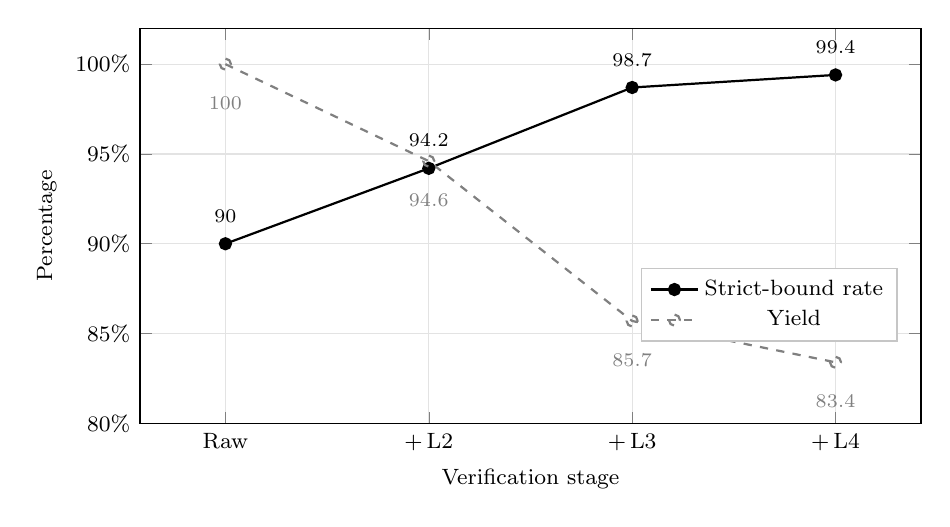
\begin{tikzpicture}
\begin{axis}[
  width=11.5cm, height=6.6cm,
  xtick=data,
  symbolic x coords={Raw,L2,L3,L4},
  xticklabels={Raw, {+\,L2}, {+\,L3}, {+\,L4}},
  ymin=80, ymax=102,
  ytick={80,85,90,95,100},
  yticklabel={\pgfmathprintnumber{\tick}\%},
  ylabel={Percentage},
  xlabel={Verification stage},
  grid=major,
  grid style={gray!22},
  legend style={at={(0.97,0.30)}, anchor=east, draw=gray!45, font=\footnotesize},
  tick label style={font=\footnotesize},
  label style={font=\footnotesize},
  enlarge x limits=0.14,
  nodes near coords,
  every node near coord/.append style={font=\scriptsize, /pgf/number format/fixed,
                                       /pgf/number format/precision=1},
]
\addplot[thick, mark=*, mark size=2pt, black,
         every node near coord/.append style={yshift=4pt}]
  coordinates {(Raw,90.0) (L2,94.2) (L3,98.7) (L4,99.4)};
\addlegendentry{Strict-bound rate}
\addplot[thick, dashed, mark=o, mark size=2pt, gray,
         every node near coord/.append style={yshift=-20pt}]
  coordinates {(Raw,100.0) (L2,94.6) (L3,85.7) (L4,83.4)};
\addlegendentry{Yield}
\end{axis}
\end{tikzpicture}
\par\vspace{0.5em}
\footnotesize\textit{Note.} Computed from the catch and false-flag targets in
Table~\ref{tab:layers}, assuming conditional independence between layers. See
the limitations noted in text: real compounding is less favourable.
\end{figure}

\subsection{Two Ways This Arithmetic Misleads}

\subsubsection{Gate Failures Are Correlated} Multiplying pass rates assumes that an
item L3 misses is no more likely to be missed by L4. In practice the assumption
fails: a subtly rephrased fact that defeats one checker tends to defeat the
others. Real compounding is therefore less favourable than the product suggests.
The composite rate must be measured end-to-end; per-layer figures drawn from
published benchmarks must never be multiplied and reported as a system result.

\subsubsection{Self-Measurement Is Circular} Filtering with detector $D$ and then
measuring with detector $D$ returns approximately 100\% by construction. The
reported SBR must be computed on a held-out, human-labelled set that the filter
never touched.

\subsection{A Calibrating Observation}

On LLM-AggreFact, an aggregation of eleven fact-checking datasets, the current
leading model attains approximately 77.4\% balanced accuracy
\parencite{bespoke2024minicheck}. That is the state of the art on hard,
adversarial grounding. The SEGS verification task is considerably easier---a
single-sentence claim tested against one 1,200-character chunk drawn from the
same document---so measured performance should be substantially better. The
observation is nonetheless the reason to measure rather than assume, and the
reason a reported figure of 99.9\% should be treated as evidence of a
measurement error.

%==============================================================================
\section{Selecting an Entailment Verifier}

Table~\ref{tab:verifiers} compares candidate L3 models. All run locally and none
requires the generation API.

\begin{table}[htbp]
\caption{Candidate Factual-Consistency Models for Layer L3}
\label{tab:verifiers}
\small
\begin{tabular}{@{}l r L{5.4cm} l@{}}
\toprule
Model & Size & Reported strength & Licence \\
\midrule
HHEM-2.1-open & 0.1\,B & Exceeds GPT-3.5-Turbo by 4.4, 5.9, and 18.1 balanced-accuracy points on AggreFact-SOTA, RAGTruth-Summ, and RAGTruth-QA; marginally exceeds GPT-4 on all three & Apache 2.0 \\
\addlinespace
MiniCheck-FT5 & 0.77\,B & GPT-4-level fact-checking at approximately 400$\times$ lower cost; trained to verify claims requiring synthesis across sentences & Apache 2.0 \\
\addlinespace
Bespoke-MiniCheck-7B & 7\,B & Leads the public LLM-AggreFact leaderboard at 77.4\% balanced accuracy & Open weights \\
\addlinespace
AlignScore & 0.35\,B & Unified alignment function trained across 15 datasets and 7 task types; state of the art on SummaC and TRUE at publication & MIT \\
\addlinespace
SummaC-ZS / -Conv & 0.4\,B & Established the sentence-level NLI aggregation method on which later work builds & Apache 2.0 \\
\bottomrule
\end{tabular}
\par\vspace{0.5em}
\footnotesize\textit{Note.} Sources: HHEM \parencite{vectara2024hhem}; MiniCheck
\parencite{tang2024minicheck}; Bespoke-MiniCheck \parencite{bespoke2024minicheck};
AlignScore \parencite{zha2023alignscore}; SummaC \parencite{laban2022summac}.
HHEM-2.1-open is recommended as the initial L3 gate on grounds of size and
licence; Bespoke-MiniCheck-7B is better suited to L4 adjudication than to the
per-item L3 gate. SummaC is included for background and is not recommended for
deployment.
\end{table}

\subsection{A Language Constraint}

HHEM-2.1-open is English-only; multilingual support is confined to the
commercial tier, and the model card does not confirm Vietnamese among the
supported languages \parencite{vectara2024hhem}. MiniCheck and AlignScore are
likewise English-trained. Because the SEGS sample corpus and the fallback
generator's stopword list are Vietnamese, deployment on Vietnamese source
documents requires either a multilingual NLI checker built on mDeBERTa or an LLM
judge at L3. This is an architectural decision with a materially different cost
profile, not a configuration value, and should be settled before L3 is
implemented.

%==============================================================================
\section{Measurement and Reporting Protocol}

A rate is only as informative as the sample behind it. The protocol requires a
calibration set of 300--400 generated items labelled by hand as grounded or
ungrounded, judged against the cited chunk alone. This set serves three
functions: it sets the L3 decision threshold, it estimates each layer's catch
and false-flag rates, and it is the only surface on which the headline SBR may
legitimately be computed.

\subsection{Sample Size Determines the Permissible Claim}

Rates near unity require interval estimation that does not rely on the normal
approximation. The Wilson score interval \parencite{wilson1927probable} is
appropriate here and is recommended over the Wald interval precisely in this
regime---small $n$, proportion near a boundary---where Wald coverage degrades
severely \parencite{brown2001interval}.

At $n = 200$ with two observed failures, an SBR of 99.0\% carries a 95\% Wilson
interval of approximately $[96.4\%, 99.7\%]$: a true rate of 96\% cannot be
excluded. At $n = 400$ with four failures the interval tightens to approximately
$[97.2\%, 99.4\%]$. The most economical route to a defensible headline figure is
the rule of three: zero failures observed in 300 labelled items bounds the error
rate at 1\%, licensing the statement that the strict-bound rate is at least 99\%
at 95\% confidence.

\subsection{Reporting}

The interface should present the measurement rather than a slogan: the rate, its
confidence interval, the sample size, the verifier and threshold used, and the
date of last calibration. Three consequent revisions to the existing system cost
nothing to make.

First, the assertion that SEGS ``eliminates hallucination entirely'' should be
withdrawn. No verification architecture supports it, and it is falsifiable by a
single counterexample. The statement that every item is checked against its
source and that unverifiable items are never displayed is both stronger and
true.

Second, the simulated analysis log---which reports a model, a temperature, and
attention-masking operations that do not correspond to the executing
system---should be replaced. Once L2--L4 exist, genuine events are available to
stream: items generated, gates failed, items regenerated.

Third, the evidence span should be displayed rather than only the citation code.
Highlighting the exact sentence the entailment model scored converts the
citation from a scroll anchor into an audit trail, which is what the
source-attribution literature means by traceability \parencite{gao2023enabling}.

%==============================================================================
\section{Related Techniques and Their Applicability}

Four further methods appear consistently in the hallucination literature. All
are substantive; none is the first component to build for this system.

\emph{Chain-of-Verification} reports substantial gains: precision on Wikidata
list questions rising from 0.17 to 0.36, MultiSpanQA F1 from 0.39 to 0.48, and
FactScore on long-form biography generation from 55.9 to 71.4 with Llama 65B
\parencite{dhuliawala2024chain}. Those are closed-book tasks in which the model
has no source text. SEGS has the source text, and deterministic containment
checks outperform self-verification when the evidence is directly available,
which is why the method belongs at L4 on the uncertain band rather than as a
primary mechanism.

\emph{Semantic entropy} samples multiple generations, clusters them by meaning,
and measures entropy across clusters, detecting confabulation without reference
text at approximately ten times the generation cost
\parencite{farquhar2024semantic}. Because a reference text always exists in the
SEGS setting, entailment verification returns more per unit of computation.

\emph{Self-RAG} trains retrieval and critique tokens directly into the model so
that it retrieves on demand and assesses its own support
\parencite{asai2024selfrag}. It is architecturally the most complete answer and
the most expensive, requiring fine-tuning; it is appropriate as related work
rather than as an implementation target.

\emph{Knowledge-graph grounding} recurs in the educational-LLM literature as a
means of anchoring generated items to structured facts. It is well suited to
curriculum alignment across an entire syllabus and disproportionate when the
bound is a single uploaded document. For the underlying taxonomy separating
extrinsic from intrinsic hallucination, which usefully frames what SEGS is
bounding, see \textcite{bang2025hallulens}.

%==============================================================================
\section{Limitations}

The catch and false-flag rates in Table~\ref{tab:layers} are working targets
selected to illustrate the filtering arithmetic; they are not measurements of
this system and no reported result should rest on them. The projection in
Figure~\ref{fig:filtering} assumes conditional independence between layers, an
assumption known to be violated in the direction that makes real performance
worse. Detector performance figures are drawn from vendor model cards and
benchmark leaderboards rather than independent replication, and the Vectara
leaderboard in particular is a live resource whose figures represent a snapshot
at the time of writing. Finally, the entire proposal is specified but
unimplemented: no component described here has been built or evaluated within
SEGS, and the 90.0\% baseline used throughout is an assumed starting point
rather than a measured property of the current pipeline.

%==============================================================================
\section{Conclusion}

The distance between SEGS's stated claim and its implemented behaviour is the
distance between a model reporting on itself and a system measuring its output.
Closing it does not require the most sophisticated available technique. It
requires, in order: deterministic checks that cost nothing and convert an
ornamental flag into a measurement; an entailment model small enough to run on
CPU; a discard-and-regenerate loop that exploits the one structural advantage
exam generation holds over summarization; and a hand-labelled calibration set
large enough to make the resulting number defensible. Under the working targets
assumed here, that sequence carries a 90.0\% baseline to 99.4\% at a yield cost
of roughly one discarded item in six---and, more importantly, produces a figure
that can be stated with an interval attached.

\printbibliography

\end{document}
